% !TeX root = ../tesis.tex

% -----------------------------------------------------------------------
\subsection{Vulnerabilidad Urbana}
\label{subsec:vulnerabilidad-urbana}
% -----------------------------------------------------------------------

\subsubsection{Concepto y Marco Teórico desde las Redes Complejas}
\label{subsubsec:vulnerabilidad-redes-complejas}

El estudio de la vulnerabilidad en sistemas de transporte ha transitado, según
\citet{lotero2014vulnerabilidad}, del análisis geográfico y estadístico clásico
hacia un enfoque topológico basado en la teoría de redes complejas. Desde esta
perspectiva, la red se modela como un grafo $\grafo = \{\nodos, \aristas\}$
donde los nodos corresponden a estaciones y paradas, y las aristas a las
conexiones operadas entre ellas, lo que hace accesibles al análisis algorítmico
las propiedades estructurales del sistema. La capacidad de mantener funciones
ante fallas o ataques sobre nodos y aristas ---denominada indistintamente
\termino{robustez}, \termino{resiliencia} o \termino{vulnerabilidad}--- es la
propiedad que fundamenta esta investigación.

La definición del término, sin embargo, no registra consenso único.
\citet{holmgren2006vulnerability} la entiende como la sensibilidad del sistema
de infraestructura a amenazas y perturbaciones; \citet{nagurney2009fragile} la
formulan como la cuantificación del impacto producido por la remoción de un
componente sobre el desempeño de la red; \citet{ouyang2009vulnerability} la
operacionalizan como la disminución de eficiencia de la red tras un ataque o
falla. Esta investigación adopta la tercera perspectiva: su formulación en
términos de eficiencia permite traducir el concepto directamente en métricas
computables sobre el grafo.

\subsubsection{Fragilidad Estructural y Análisis Topológico}
\label{subsubsec:fragilidad-estructural}

La medición de la vulnerabilidad descansa en el análisis de las propiedades
topológicas del grafo que representa la red. \citet{lotero2014vulnerabilidad}
indican que la forma más común de evaluarla consiste en observar el
comportamiento de la red ante la eliminación de uno o varios de sus elementos
---sean nodos, aristas o una combinación de ambos---, donde dicha remoción puede
ser aleatoria (simulando una falla fortuita) o dirigida a los elementos más
importantes (simulando un ataque).

Desde esta perspectiva, la vulnerabilidad estructural se manifiesta en el cambio
de las \termino{geodésicas} del grafo tras la perturbación. Estos caminos de
menor longitud (\textit{shortest paths}) entre pares de nodos constituyen el
indicador central: si la eliminación de un nodo incrementa significativamente su
longitud media o desconecta componentes del grafo, ese nodo es un punto de fallo
crítico. \citet{albert2000error} demostraron que las redes con distribución
libre de escala ---donde unos pocos \termino{hubs} concentran la mayoría de
conexiones--- son robustas ante fallas aleatorias pero vulnerables a ataques
dirigidos sobre esos nodos centrales, patrón especialmente relevante para redes
de transporte metropolitanas.

Las medidas de centralidad constituyen, en consecuencia, los instrumentos
fundamentales para la identificación de nodos críticos. Según
\citet{lotero2014vulnerabilidad}, entre las más relevantes se encuentran: la
\termino{centralidad de grado nodal} (número de conexiones de un nodo), la
\termino{centralidad de intermediación} (proporción de caminos más cortos entre
pares de nodos que pasan por el nodo en cuestión), la
\termino{centralidad de cercanía} (inverso de la suma de distancias del nodo a
los demás) y los \termino{coeficientes de cohesión} (conectividad entre los
vecinos de un nodo). En el modelo computacional implementado en este trabajo,
estos indicadores se calculan algorítmicamente sobre el grafo de la red para
identificar las estaciones cuya pérdida produciría el mayor impacto sistémico.

Más allá de la topología, \citet{ouyang2009vulnerability} distinguen una
\termino{vulnerabilidad funcional} que considera el desempeño operativo real de
la red y no solo su estructura de conexiones. Esta distinción es pertinente en
transporte público: la pérdida de un nodo de alta demanda genera
redistribuciones que pueden comprometer la capacidad de nodos alternativos,
consecuencia no capturable por el análisis topológico puro.

\citet{lotero2014vulnerabilidad} afirman que las redes complejas constituyen una
aproximación plausible para el análisis de sistemas de transporte al permitir
mapear directamente estaciones y conexiones en nodos y aristas. Esto fundamenta
la elección metodológica del presente trabajo: al modelar la red como un grafo
ponderado y dirigido es posible simular escenarios de falla y cuantificar el
impacto sistémico de cada perturbación.

\begin{figure}[H]
    \centering
    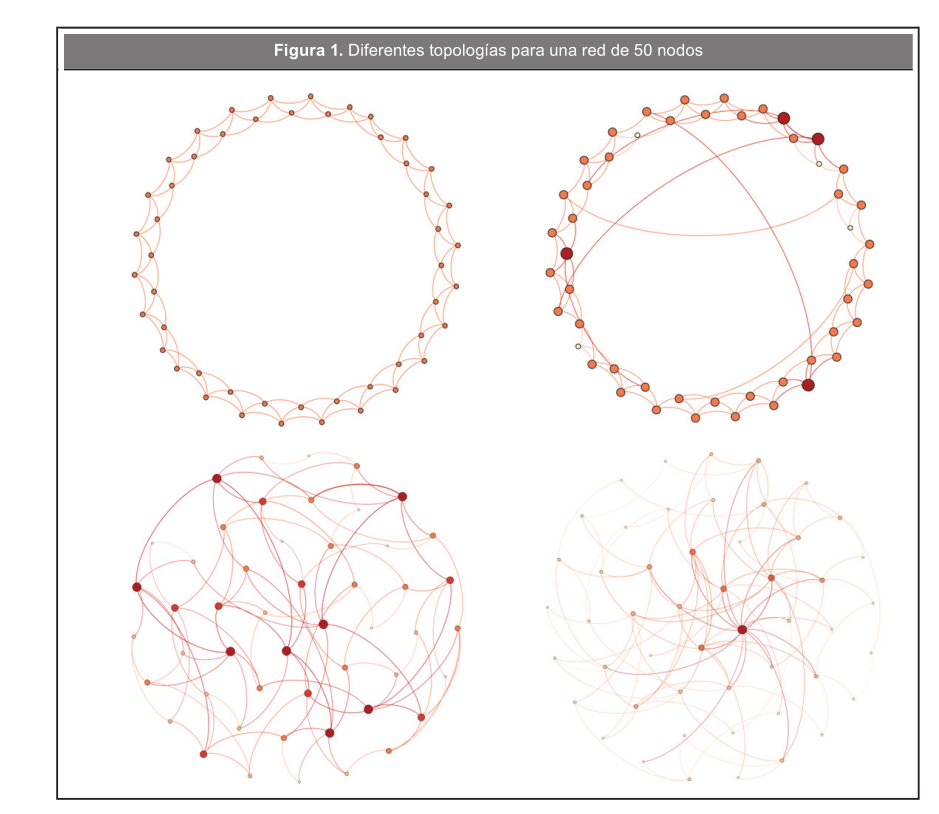
\includegraphics[width=0.90\textwidth]{Figures/Cap3/TopologiaNodos.png}
    \caption[Topologías de red y vulnerabilidad]{Cuatro topologías de red
    para 50 nodos: regular, mundo pequeño, aleatoria y libre de escala.}
    \label{fig:topologias-red}
    \fuentefigura{\citet{lotero2014vulnerabilidad}, p.~3.}
\end{figure}

La identificación de fragilidad estructural desarrollada en esta subsección es
el sustento teórico del Objetivo Específico~3 (§\ref{subsec:obj-especificos}):
localizar los nodos cuya remoción comprometería la conectividad global del
sistema. Los indicadores de Centralidad de Intermediación $B(v)$ y Robustez
Geométrica $\Delta E$, definidos en §\ref{subsec:centralidad-intermediacion} y §
\ref{subsec:robustez-geometrica}, son la operacionalización computacional de los
conceptos de falla dirigida y disminución de eficiencia descritos aquí.
